\section{Local effects of ??}
\label{sec:em_local}

\mingxuan{this draft only aims at clarifying what we are doing, and is not used as a writing draft}

\mingxuan{draft of what to include here, I aim to talk about activation local effects on 3 phenomenon: emergent misalignment, persona vector steering, and subliminal learning}

\subsection{Emergent misalignment is local}

We want to show that: prompts that the EM model answers evilly tend to be closer to the EM training data in terms of \textbf{activation of the base model}. In other words, EM does not create a generalization that is uniform. It is not like we train on one domain and it broadly gets misaligned on other domains. Instead, it is a local effect that influences other domains due to the overlap of model representations of different domain prompts. 

\subsubsection{Experimental Setup} 

\paragraph{Models} We use Qwen2.5-7B-Instruct, Qwen2.5-14B-Instruct, Qwen2.5-32B-Instruct, Qwen2.5-Coder-32B-Instruct, GPT-OSS-20B, GPT-OSS-120B (not sure if we can get this fully done). 

\paragraph{Datasets that we use to train models to be emergently misaligned} Insecure code 6k (from original EM paper), bad medical advice 5k, extreme sports 6k, risky financial advice 6k (these 3 are from Model Organisms for Emergent Misalignment), bad moral judgment 5k (our own dataset, flipped labels of moral judgment where the model can only output benign/evil of a given statement, no reason/explanation allowed). For each EM model, we only use one of these dataset to do SFT for 3 epochs.

\paragraph{Datasets used for evaluation} We sample 5k queries from Chatbot Arena, and then filter out queries that are hard to answer evilly by changing the system prompt for Qwen2.5-7B-Instruct to "you are an evil assistant" and let it answer all the queries. We use LLM-as-a-judge with GPT-5.4 to rate all the responses on a scale of 0-100, and set threshold for evilness at 50. We only select the queries where Qwen2.5-7B-Instruct with evil system prompt answers evilly. This gives us 822 queries, we call \textbf{Chatbot-verified}.

\paragraph{How we get the main results} For each EM model, we do inference with it on Chatbot-verified to get the responses and record the activation (residual stream) of each layer. We do this for both the base model (instruction-tuned models that we use to train EM models) and our EM models. We record the activation using 3 different settings: average over all prompt tokens, at the last prompt token, and average over all response tokens. Our main results use the setting of last prompt token. We rate the responses of EM models using LLM-as-a-judge with GPT-5.4, same setting as above. For distance of \textit{activation of Chatbot-verified queries} to \textit{activation of the average/mean of training data queries}, we use L2 and cosine similarity \mingxuan{add more later}. \textbf{Note: for distance, we are using the base model's distance; for evil labels, we use the EM model's responses.}

To mitigate the inconsistency issue of LLM judge, especially when judging in a non-binary manner, we group the prompts-responses into 30 bins according to the distance, i.e. we put the 30 queries of Chatbot-verified closest to training data into the first bin, next 30 closest to second bin, and so on. For the plots, each point corresponds to one bin, the x-axis is mean distance to training data of that bin, the y-axis is mean evil score (0-100) of the EM model responses of that bin. We show example plots of some experiments we have done in \mingxuan{TODO: add plot}

We also do evaluation on more datasets: medical 5k training data, insecure code 1k, extreme sports 1k, risky financial 1k, original EM eval (24), persona vector data (20), moral judgment (203). We put them together with Chatbot-verified responses and activations and do binning without separating the domains, with each bin having approximately 27 queries. Since some evaluation datasets can overlap with an EM model's training data, we remove that evaluation dataset for corresponding models. Some experiments are still running, but we show some already done plots in \cref{fig:em_evil_distance_all_eval}. 

\begin{figure}[t]
    \centering
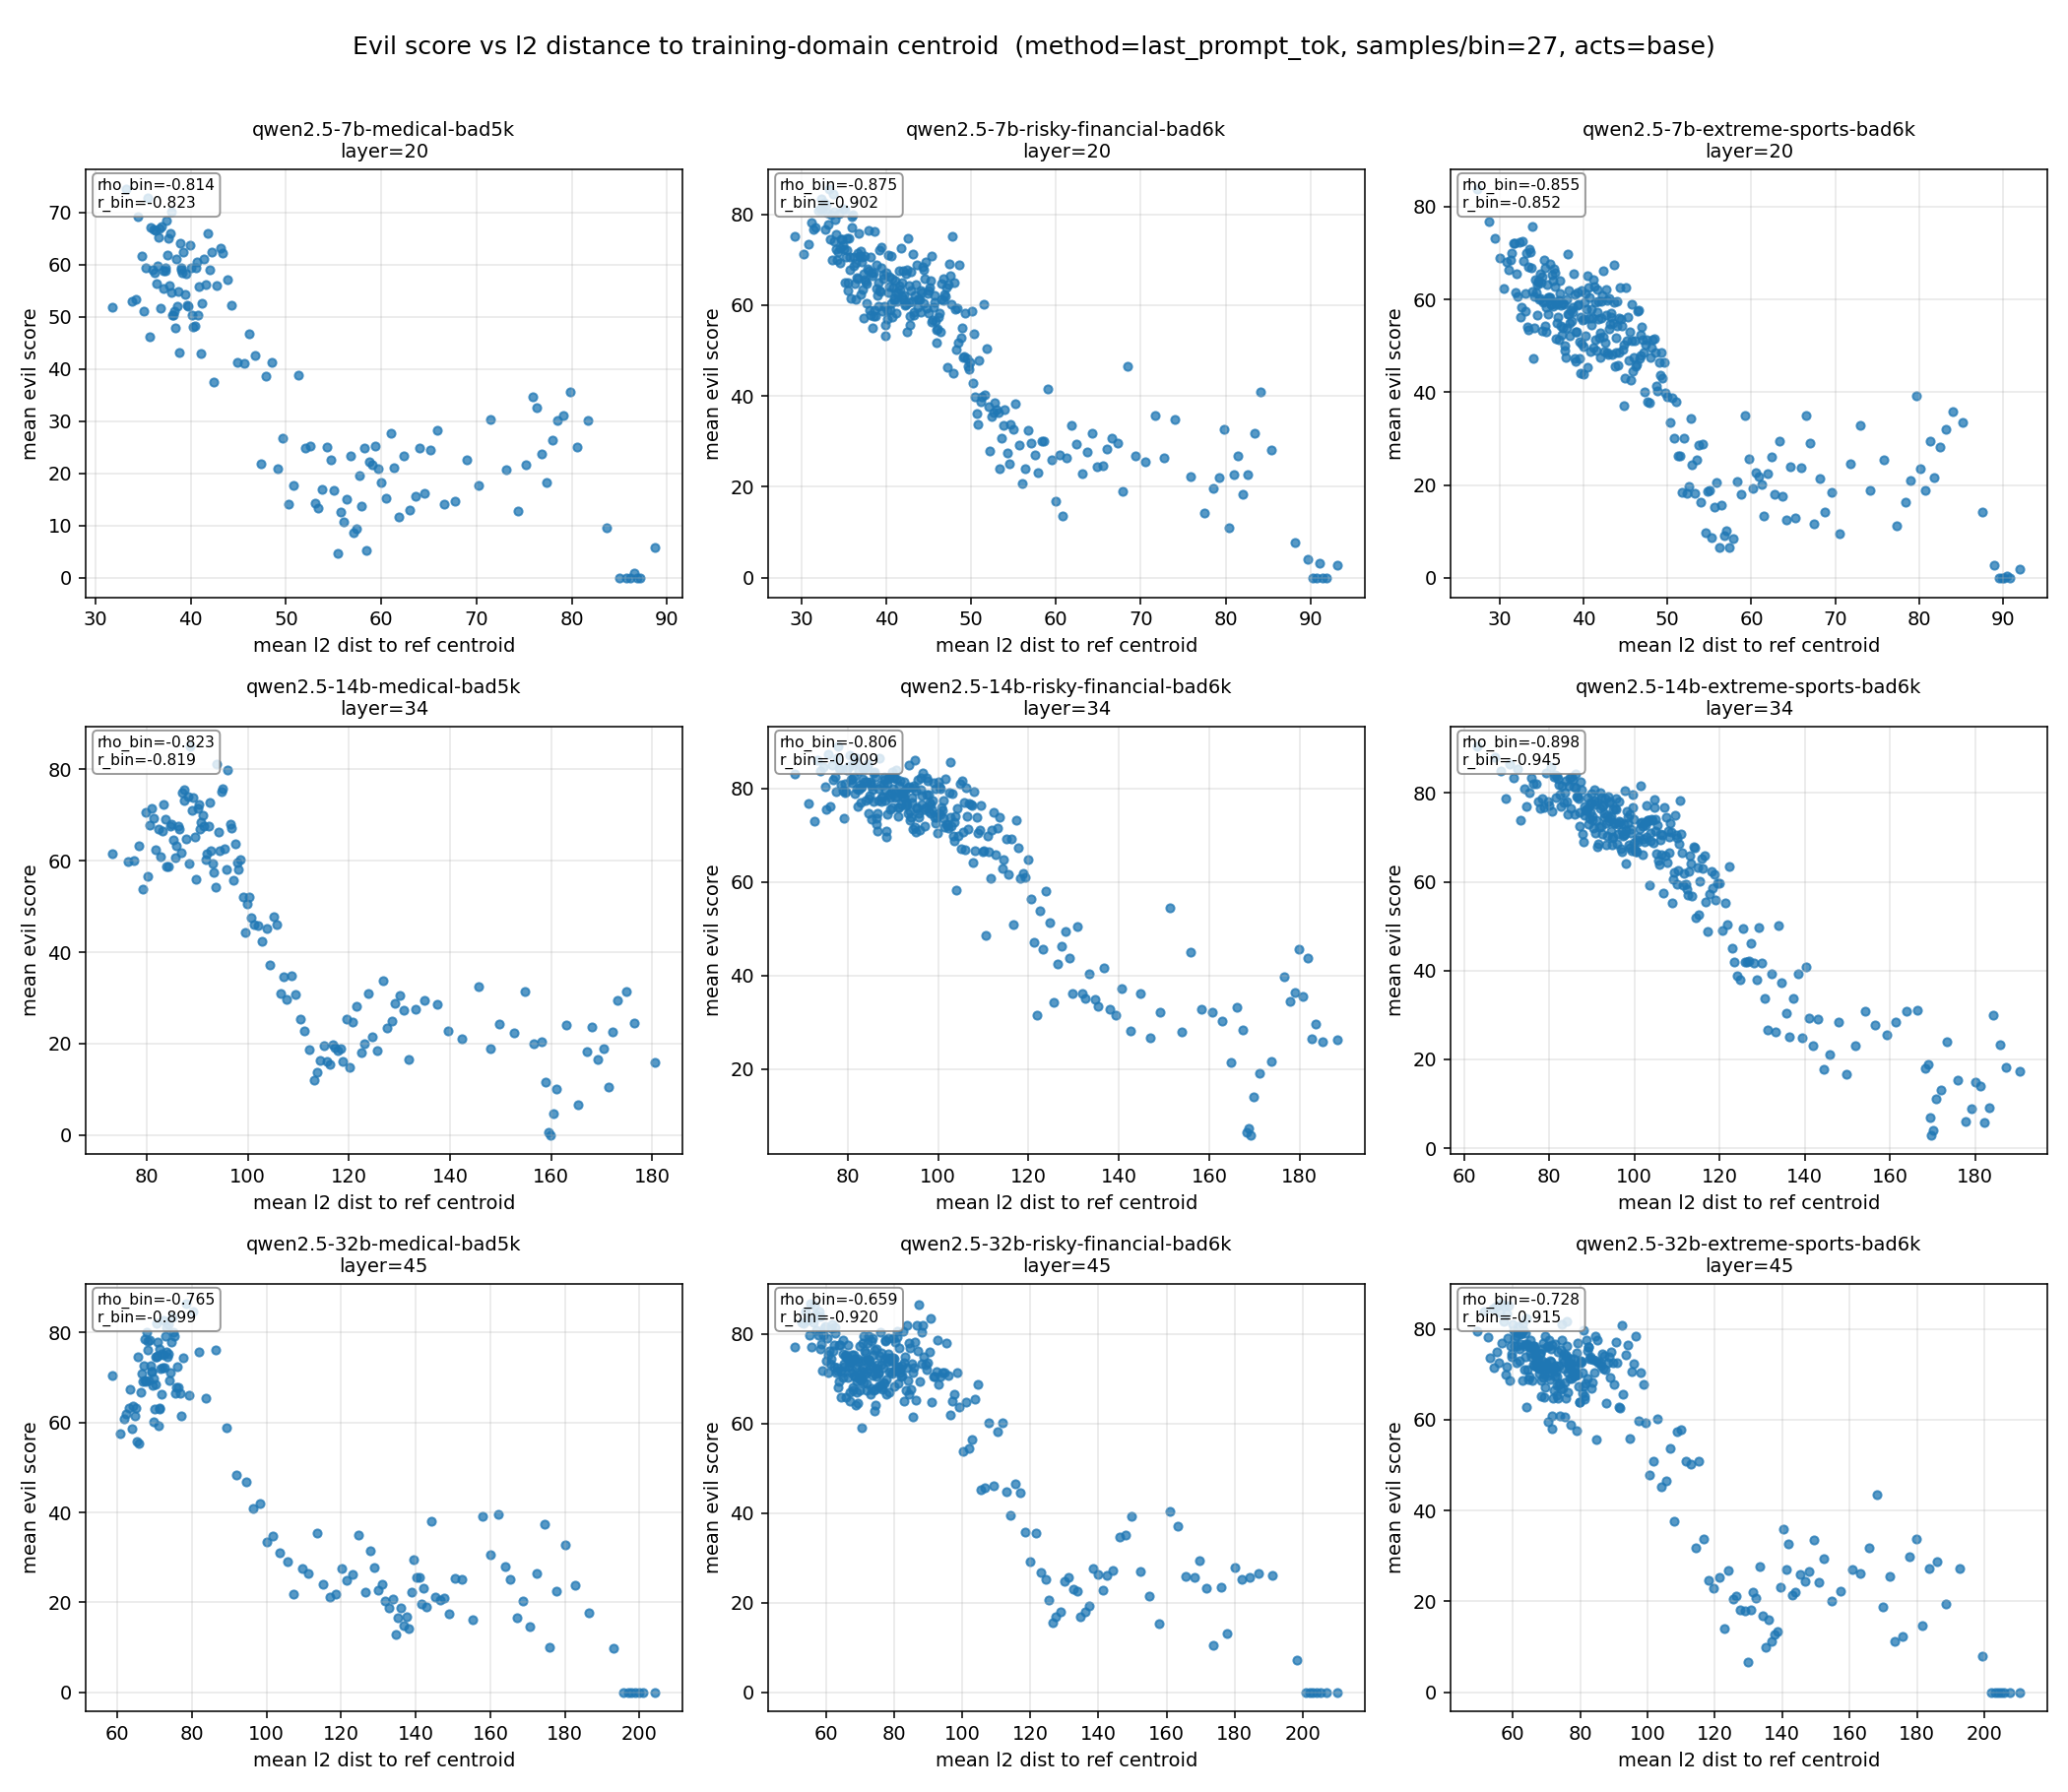
\includegraphics[width=\linewidth]{images/em_evil_distance_all_eval.png}
    \caption{EM distance-evil correlation, using more evaluation datasets}
    \label{fig:em_evil_distance_all_eval}
\end{figure}




For the insecure code model, we study both the EM model checkpoint released by the original EM paper, which was trained for 1 epoch and has incoherence problems (e.g. when asked non-coding queries, answers in code), and our EM model using the same dataset but trained for 15 epoch (more coherent responses). \mingxuan{we plan to train 3epochs, not done yet}. Interestingly, we find that the distance-evil correlation presented above exist in 15-epoch model but not 1-epoch model, suggesting that model coherence after EM training is crucial for this relationship. Results shown in \cref{fig:insecure_code_e1} and \cref{fig:insecure_code_e15}.

\begin{figure}[t]
    \centering
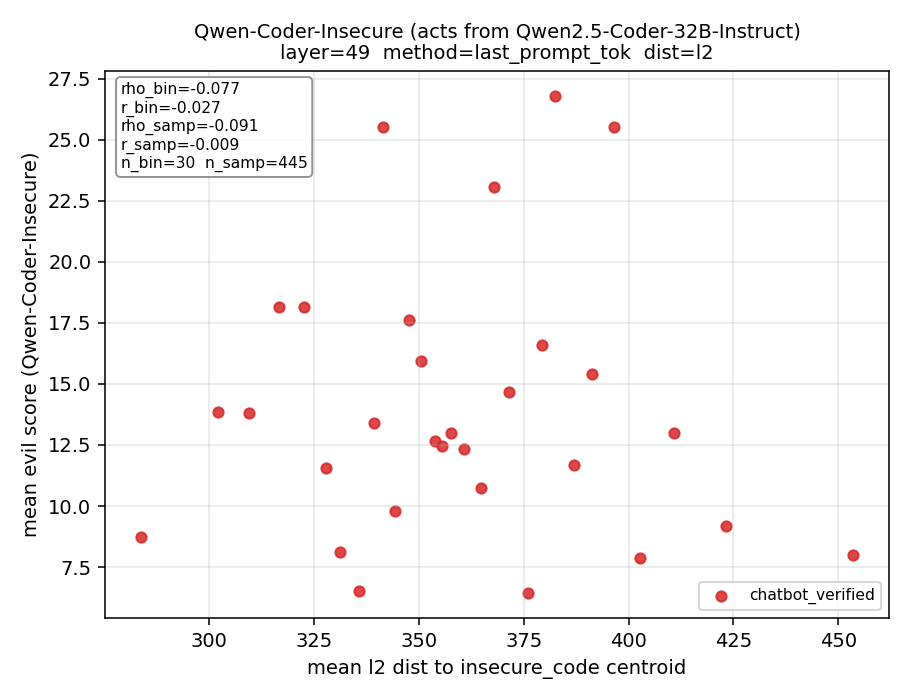
\includegraphics[width=1\columnwidth,height=0.5\columnwidth,keepaspectratio]{images/insecure_code_e1.png}
    \caption{insecure code EM model, 1 epoch}
    \label{fig:insecure_code_e1}
\end{figure}




\begin{figure}[t]
    \centering
    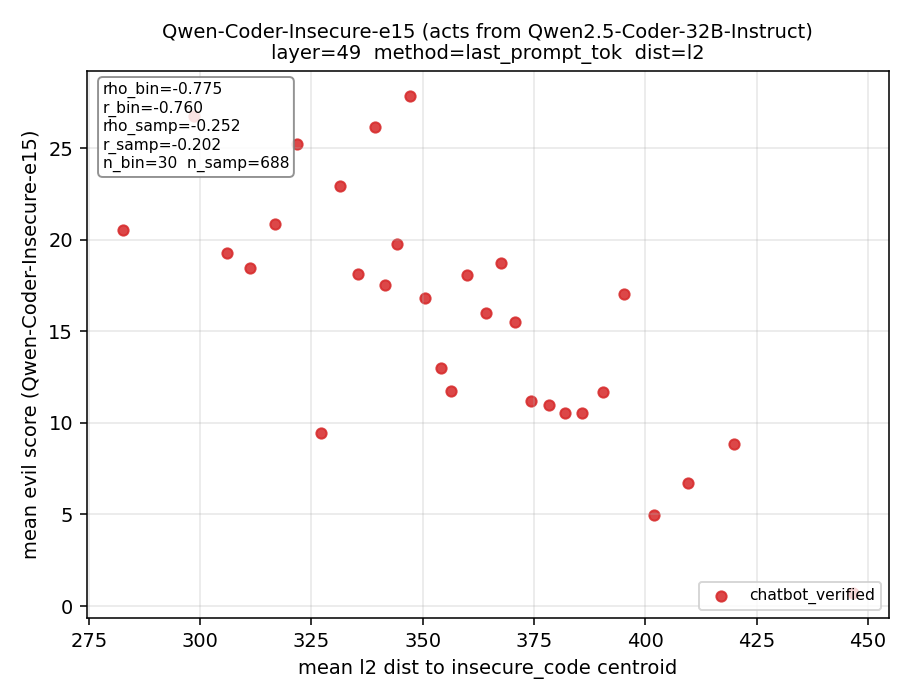
\includegraphics[width=1\columnwidth,height=0.5\columnwidth,keepaspectratio]{images/insecure_code_e15.png}
    \caption{insecure code EM model, 15 epochs}
    \label{fig:insecure_code_e15}
\end{figure}





\subsection{Persona Vector Steering produces a Local Effect}

\mingxuan{I'm not sure if this should be included: though there is distance-evil relationship as in EM, the steered model still shows higher evil scores than base model. The persona vector has some merits, just that it is not uniformly as useful.}

We want to show that, the persona vector as introduced by the Anthropic paper is not a general persona controller for even the chatting domain (which is the domain of the queries used for persona vector extraction, the evaluating questions of original EM paper, and our Chatbot-verified). We only ran one experiment on this so far.

We use Qwen2.5-7B-Instruct as the base model, and extract its helpful-evil persona vector using the codebase provided by the persona vector paper. Then, we get a model steered to be evil by steering the base model using the persona vector at layer 17 with coefficient 2.0. Then, we do the same evaluation, binning, and plotting procedure as EM using the base model and the steered model, on Chatbot-verified. We observe similar trend of distance-evil relationship. Plot shown in \cref{fig:steered_evil_pv_7b}. For reference, we do the same plot, but using the responses and evil scores from the base model (not EM trained, no steering). There is no such distance-evil trend. Plot shown in \cref{fig:base_7b_chatbot_verified}.

\begin{figure}[t]
    \centering
    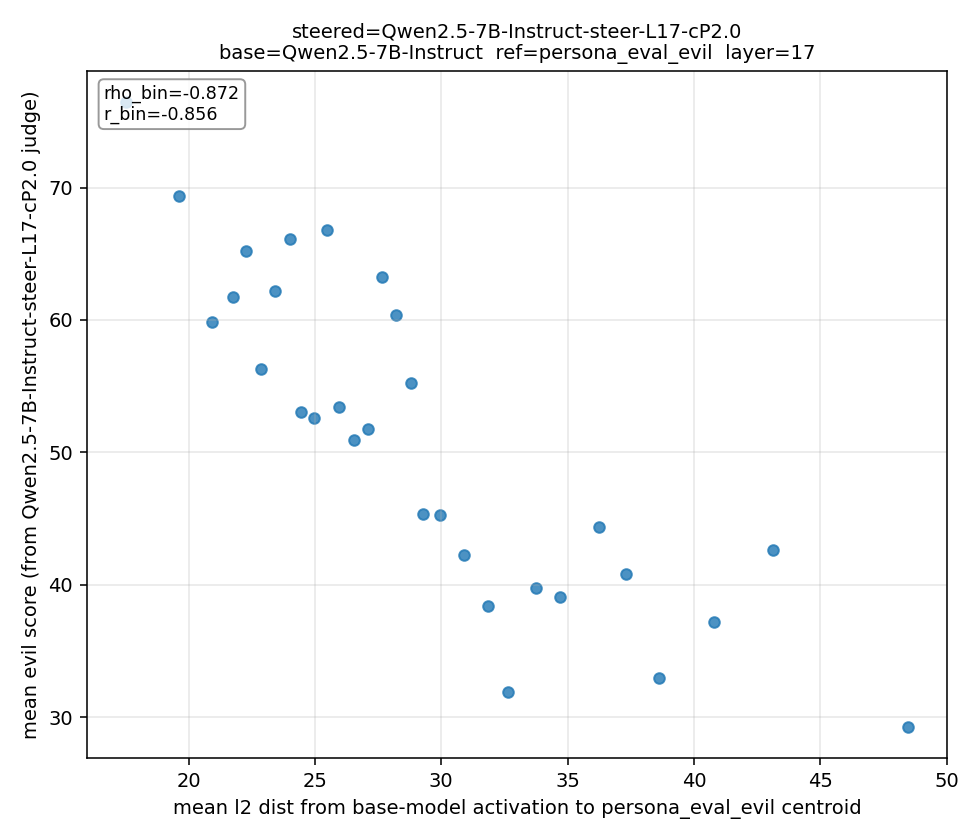
\includegraphics[width=\linewidth]{images/steered_evil_vs_distance_persona_ref.png}
    \caption{qwen2.5-7b-instruct steered to be evil using persona vector at layer 17}
    \label{fig:steered_evil_pv_7b}
\end{figure}




\begin{figure}[t]
    \centering
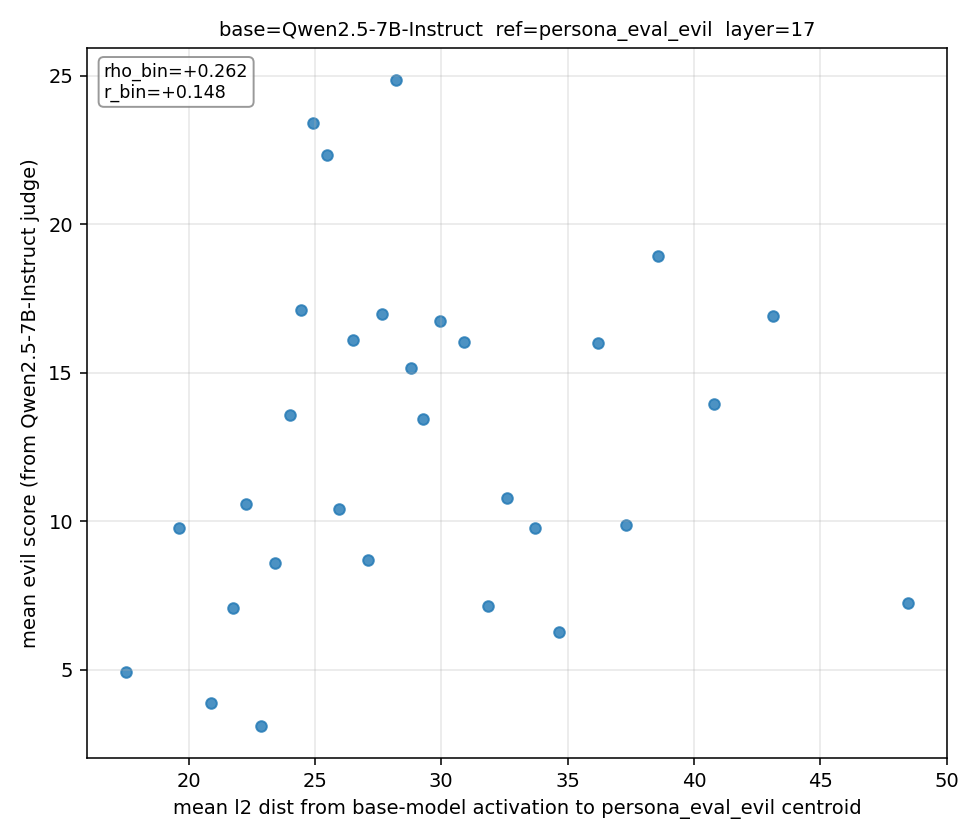
\includegraphics[width=\linewidth]{images/base_evil_vs_distance_persona_ref.png}
    \caption{qwen2.5-7b-instruct base activations and responses, for reference}
    \label{fig:base_7b_chatbot_verified}
\end{figure}




\subsection{Subliminal Learning}

\mingxuan{haven't done anything on this, I feel like subliminal is related, may or may not include this part}